%%%%%%%%%%%%%%%%%%%%%%%%%%%%%%%%%%%%%%%%%
% Large Colored Title Article
% LaTeX Template
% Version 1.1 (25/11/12)
%
% This template has been downloaded from:
% http://www.LaTeXTemplates.com
%
% Original author:
% Frits Wenneker (http://www.howtotex.com)
%
% License:
% CC BY-NC-SA 3.0 (http://creativecommons.org/licenses/by-nc-sa/3.0/)
%
%%%%%%%%%%%%%%%%%%%%%%%%%%%%%%%%%%%%%%%%%

%----------------------------------------------------------------------------------------
%	PACKAGES AND OTHER DOCUMENT CONFIGURATIONS
%----------------------------------------------------------------------------------------

\documentclass[DIV=calc, paper=a4, fontsize=12pt]{scrartcl}	 % A4 paper and 12pt font size

\usepackage{geometry}
\usepackage{multicol}
\usepackage{sectsty} % Enables custom section titles
\usepackage{minitoc}
%\usepackage{multicol} %Enables multiple columns and additional commands
\usepackage[utf8]{inputenc}
\usepackage[english]{babel} % English language/hyphenation
\usepackage[protrusion=true,expansion=true]{microtype} % Better typography
\usepackage{amsmath,amsfonts,amsthm} % Math packages
\usepackage[svgnames]{xcolor} % Enabling colors by their 'svgnames'
\usepackage[hang, small,labelfont=bf,up,textfont=it,up]{caption} % Custom captions under/above floats in tables or figures
\usepackage{booktabs} % Horizontal rules in tables
\usepackage{fix-cm}	 % Custom font sizes - used for the initial letter in the document
\usepackage{graphicx} %Use graphics and figures			
\usepackage{gensymb} %More symbols
\usepackage{float}
\usepackage{fixltx2e}
\usepackage[toc,page]{appendix}

\allsectionsfont{\usefont{OT1}{phv}{b}{n}} % Change the font of all section commands

\usepackage{fancyhdr} % Needed to define custom headers/footers
\pagestyle{fancy} % Enables the custom headers/footers
\usepackage{lastpage} % Used to determine the number of pages in the document (for "Page X of Total")

\usepackage{tcolorbox}

% Headers - all currently empty
\lhead{}
\chead{}
\rhead{}

% Footers
\lfoot{}
\cfoot{}
\rfoot{\footnotesize Page \thepage\ of \pageref{LastPage}} % "Page 1 of 2"

\renewcommand{\headrulewidth}{0.0pt} % No header rule
\renewcommand{\footrulewidth}{0.4pt} % Thin footer rule

\fancyfootoffset{0mm}

\usepackage{lettrine} % Package to accentuate the first letter of the text
\newcommand{\initial}[1]{ % Defines the command and style for the first letter
\lettrine[lines=2,lhang=0.3,nindent=0em]{
\color{DarkBlue}
{\textsf{#1}}}{}}

%----------------------------------------------------------------------------------------
%	TITLE SECTION
%----------------------------------------------------------------------------------------

\usepackage{titling} % Allows custom title configuration

\newcommand{\HorRule}{\color{DarkBlue} \rule{\linewidth}{1pt}} % Defines the gold horizontal rule around the title

\pretitle{\vspace{-30pt} \begin{flushleft} \HorRule \fontsize{22}{30} \usefont{OT1}{phv}{b}{n} \color{DarkBlue} \selectfont} % Horizontal rule before the title

\title{Biologisk skattejakt på planteten Mars \\ Prosessrapport \\ Gruppe 3} % Your article title

\posttitle{\par\end{flushleft}\vskip 0.5em} % Whitespace under the title

\preauthor{\begin{flushleft}\large \lineskip 0.5em \fontsize{12}{15} \usefont{OT1}{phv}{b}{sl} \color{DarkBlue}} % Author font configuration

\author{Ingelin Garmann, Simen L. Hegge, Karsten Olav Kjensmo, Jonas Sandøy Misund, Martin Nordal, Anna Solveig Julia Testani\`{e}re, } % Your name

\postauthor{\footnotesize \usefont{OT1}{phv}{m}{sl} \color{Black} % Configuration for the institution name
Norges Tekniske og Naturvitenskaplige Universitet % Your institution

\par\end{flushleft}\HorRule} % Horizontal rule after the title

\date{} % Add a date here if you would like one to appear underneath the title block

%----------------------------------------------------------------------------------------
%	SECTION TITLE
%----------------------------------------------------------------------------------------

\sectionfont{\Large \MakeUppercase}

\subsectionfont{\normalfont \MakeUppercase}

%----------------------------------------------------------------------------------------
%	TEXT
%----------------------------------------------------------------------------------------

\setlength{\columnsep}{32pt}
\linespread{1.2}

\geometry{
a4paper,
total={210mm,297mm},
left=15mm,
right=15mm,
top=20mm,
bottom=20mm}

%----------------------------------------------------------------------------------------
%	IMAGES
%----------------------------------------------------------------------------------------

\graphicspath{{Bilder/}}
\floatstyle{boxed}
\restylefloat{figure}

%----------------------------------------------------------------------------------------
%	APPENDIX
%----------------------------------------------------------------------------------------

\renewcommand\appendixpagename{Vedlegg}
\renewcommand\appendixtocname{Vedlegg}

%----------------------------------------------------------------------------------------

\begin{document}
\maketitle % Print the title

\thispagestyle{fancy} % Enabling the custom headers/footers for the first page 

%----------------------------------------------------------------------------------------
%	ABSTRACT
%----------------------------------------------------------------------------------------

% The first character should be within \initial{}

%----------------------------------------------------------------------------------------
%	ARTICLE CONTENTS
%----------------------------------------------------------------------------------------

\section*{Forord}

\begin{multicols}{2}


\end{multicols}

%----------------------------------------------------------------------------------------

\section*{Sammendrag}

\begin{multicols}{2}

\end{multicols}

%----------------------------------------------------------------------------------------

\pagebreak
\renewcommand{\contentsname}%
	{Innhold}

\tableofcontents

%----------------------------------------------------------------------------------------

\pagebreak
%\section{Innledning}

\section{Introduksjon til EiT}

Eksperter i team (EiT) er et obligatorisk emne for studenter som tar mastergrad på NTNU. 
Som forklart i emnebeskrivelsen\cite{eitlaeringsmaal} av faget, er hensikten med EiT å være et yrkesforberedende fag hvor studenten får erfaring med å arbeide i en tverrfaglig gruppe.
Emnet er utviklet på bakgrunn av at det i arbeidslivet ofte skal samarbeides i tverrfaglige prosjekter, en setting de færreste studenter har erfaring med før EiT.
Innsikt i gruppedynamikk skal læres ved å reflektere over og diskutere oppgaver, både innenfor et faglig prosjekt og en samarbeidsprosess.
Målet er at studentene skal bli bedre kjent med seg selv som en del av en gruppe, og hvordan gruppen og studenten påvirker hverandre.
Studenten skal utvikle sine samarbeidende egenskaper, bli komfortabel i å kommunisere, og lære hvordan å unngå samt håndtere konflikter.
Et like viktig mål med emnet er at studentene skal kunne formidle og anvende sin egen kunnskap og lære fra andres fagområder.
Læringsmålet innen samarbeid og læringsmålet innen tverrfaglig arbeid skal presenteres i to separate rapporter som vektes likt i det resulterende karakterresultatet.
\\

%\begin{multicols}{2}

%\end{multicols}

%----------------------------------------------------------------------------------------

\section{Landsbyen og gruppen}

%\begin{multicols}{2}


\subsection{Landsbyen - Biologisk skattejakt på planeten Mars}

Landsbyen - Biologisk skattejakt på planeten Mars - består av rundt 20 medlemmer.
Disse er fordelt på tre grupper som hver for seg skal jobbe med de samme spørsmålene:
{\textit{Hva kan vi finne av liv/spor av liv på planeten Mars?
Hvordan kan dette fortelle oss mer om hvordan livet oppstod på vår egen planet?
Hva forteller dette oss om liv ellers i verdensrommet?}}















\subsection{Gruppemedlemmene}

For å gi et innblikk i hvilke medlemmer gruppen består av velger vi å presentere oss selv.
I de kommende avsnittene har vi alle skrevet om oss selv; hvem vi er, hvor vi kommer fra, hvilke interesser vi har og hvilke forventninger vi hadde til Eksperter i Team (både til fag og prosess).
\\

\subsubsection{Anna}

\paragraph{Personalia}
Er 25 år gammel, født og oppvokst i Sør-Frankrike. Jeg flyttet til Norge i 2007 og bodde også et år i Berkeley, California, i fjor.
Studerer teoretisk matematikk med fordypning i kryptografi. Masteroppgaven jeg skriver handler om elektroniske stemmesystemer.

\paragraph{Forventninger til EiT}
På forhånd hadde jeg hørt flest negative holdninger til EiT.
Dette var fra andre studenter som hadde hatt faget.
Likevel hadde jeg selv en positiv innstilling til faget siden jeg ikke hadde hatt gruppearbeid tidligere i utdanningen på NTNU.
Derfor var jeg nysgjerrig på hvordan det ville være.
Jeg syntes også at det hørtes lurerikt ut å reflektere rundt samarbeidet i seg selv.
Biologisk skattejakt på planeten Mars var mitt andrevalg som landsby på grunn av fasinasjonen for romfart.
Jeg var klar over at landsbyen lå utenfor mitt fagfelt og det var spennende med en utfordring!
\subsubsection{Ingelin Garmann}

\paragraph{Personalia}
23 år, oppvokst i Bergen og bodde der til utgangen av videregående med unntak av et skoleår på utveksling i Nevada, USA.
Gjennomførte et år med førstegangstjeneste i Hæren etter videregående.
Holder på med Siv.ing grad innen Industriell kjemi med spesialisering innen Kjemisk Prosessteknologi med størst interesse for prosesskontroll og reguleringsteknikk.
Driver med CrossFit og vektløfting på fritiden.

\paragraph{Forventninger til EiT}
Jeg var veldig spent på å arbeide i en tverrfaglig gruppe med stort fokus på selve gruppedynamikken.
Et slikt fokus er fremmed for de fleste innen tekniske studier, slik at jeg forventet og håpet å få god erfaring på området.
I tillegg til erfaring ønsket jeg å lære metoder for å unngå konflikter, og ikke minst bli mer bevisst på meg selv som person i en gruppe.
I tillegg var jeg spent på hvordan jeg kunne bidra faglig og hva jeg kunne lære av andre.
Landsbyen "Biologisk skattejakt på planeten Mars" var ikke ett av mine øverste valg da interessen for biologi ikke var så stor.
Jeg hadde forventninger om å kunne benytte både kreativitet og teknologi i en problemstilling som omhandlet kolonisering og terraforming av en planet.
På tross av at jeg hadde hørt negative bemerkninger om EiT, var jeg innstilt på å få noe positivt ut av faget!
\subsubsection{Jonas Sandøy Misund}

\paragraph{Personalia}
Jeg er født i Oslo i 1992 og oppvokst i Molde fra 1998.
Jeg studerer fysikk og matematikk med spesialisering innen teknisk fysikk ved NTNU.
Mye av fritiden min går med til frivillige verv, blant annet som hovmester i Lyche, restauranten på Studentersamfundet i Trondhjem.

\paragraph{Forventninger til EiT}
Eksperter i Team er et fag jeg har hørt både positive og negative ting om siden jeg begynte på NTNU.
Alt fra innslag under revyen, til venner som har vært læringsassistenter i fag har gitt meg inntrykk av EiT.
Selv hadde jeg ikke så mange tanker om hva vi skulle drive med i EiT, men ønsket å lære noe nyttig om gruppearbeid mens jeg deltok.
Gruppearbeid i seg selv er veldig interessant og moro å drive med, så jeg gledet meg litt til å få noe mer håndfast kunnskap om nettopp dette.
Ellers er jeg, som den fysikknerden jeg er, ganske interessert i omtrent alt som foregår ute i verdensrommet.
Mars er jo nettopp noe som \textit{foregår} ute i verdensrommet.
Derfor ble "Biologisk skattejakt på planeten Mars" en av landsbyene jeg satte opp som alternativer.
\subsection{Karsten Olav Kjensmo}

\paragraph{Personalia}
25 år. Har vokst opp i bl. a. Danmark, Nigeria, Namibia og USA. Opprinnelig født i Bærum, men har har ikke gått på norsk skole eller bodd lenge i Norge før universitetstiden. Har gjennomført en bachelorgrad i informatikk, og går mastergrad i informatikk på linjen databaser og søk; hvor jeg skriver oppgave innen kunstig intelligens og webteknologi. Har derutover faglig interesse i kognitive arkitekturer og designteori knyttet til menneske-maskin interakjson. På fritiden sykler jeg på fjellet, driver med hobbybryting og knoter med datateknologi. 

\paragraph{Forventninger til EiT}
Ved fagets start var inntrykket godt. En god studiekamerat har tatt både faget og den spesifikke landsbyen før, og hadde bare gode ting og si. Det ble kommentert på den trivelige stemningen i landsbyen - noe som alle landsbyer ikke har - samt den faglige friheten knyttet til oppgaven og emnet. Det faglige trakk av flere grunner - jeg er amatør på biologifeltet, men mente ikke dette ville være et problem, da jeg trodde det ville være mange biologer på landsbyen og at jeg med datavitenskap ville kunne bringe en ny vinkel på deres felt, spesifikt med datavitenskapen knyttet til romfart og utforskningsroboter. Det sosiale var også en faktor, da det ikke er mangel på skrekkhistorier om EiT grupper (nok noe overdrevet eller selvpåført) som ikke hang sammen sosialt. Andre studiekamerater har kommentert på dette, og har mistrivdes stort, og dette var et element i avgjørelsen da jeg valgte å søke landsbyen for biologisk skattejakt på Mars. Ved fagets start var jeg altså innstillt på å lære fra andre fagfelter, samt teste meg selv i en sosial arena med et introspektivt fokus. 





\subsubsubsection*{Martin Nordal}

\paragraph{Personalia}
Er 24 år og kommer fra Oslo.
Interessen for programmering og skripting fikk meg til datateknikk-studiet, etterhvert med retning kunstig intelligens.
Har også interesse for romfart, noe som førte til at jeg søkte på denne EiT-landsbyen.

\paragraph{Forventninger til EiT}
Forhåndsinntrykket til EiT har til dels vært basert på beretninger fra eldre personer som har hatt faget tidligere.
Det gjentakende i deres beretninger har vært at faget inneholder for mye obligatoriske aktiviteter som ikke har vært oppfatta som nyttig, mens det ble altfor liten tid til å arbeide med eventuelle prosjekter eller de endelige rapportene.
Gjennom studiene så langt har jeg selv vært med på mye gruppearbeid.
Det har stort sett vært trivelig og produktivt, men enkelte gruppesammensetninger, og kanskje spesielt de store gruppene, ikke har fungert så bra.
EiT kunne derfor være behjelpelig for å lære hvordan man i fellesskap skal takle menneskelige utfordringer i en gruppe.
\subsubsection{Simen Løvøy Hegge}

\paragraph{Personalia}
Jeg er 23 år gammel og kommer fra Kunes, en liten plass midt i Finnmark med 30 innbyggere.
Bor for tiden i Trondheim sammen med min samboer og vår sønn på snart to år.
Vi venter vårt andre barn høsten 2015.
Jeg har en bachelorgrad innen allmenn bygg fra Høgskolen i Narvik, og bygger nå på med 2-årig master på bygg og miljøteknikk, retning konstruksjon ved NTNU.

\paragraph{Forventninger til EiT}
Høgskolen i Narvik hadde ingen fag som het (eller minnet om) EiT.
Jeg hadde derfor aldri hørt om faget før jeg begynte på NTNU.
Hørte fa en del negative ting om faget fra medelever her på NTNU, men lot ikke dette påvirke mitt inntrykk. 
Det hørtes ut som et nyttig fag med tanke på samarbeid.

Denne landsbyen var ikke førstevalget siden den ikke treffer fagfeltet mitt.
Ordet "biologi" føles langt fra fagfeltet konstruksjon, men utforsking av Mars pirret romfartsinteressen min.
Denne landsbyen ble derfor andrevalget.

%\end{multicols}

%----------------------------------------------------------------------------------------

\section{Metodebeskrivelse}

%\begin{multicols}{2}

\subsection{Rammeverk}

Landsbyen "Biologisk skattejakt på planeten Mars" er en langsgående landsby.
Det innebærer obligatorisk oppmøte hver onsdag i 15 uker. Før de resulterende rapportene fra prosjekt- og prosessoppgaven kan leveres, må gruppen holde en muntlig prosjektpresentasjon og delta på en prosessamtale med læringsassistenter og landsbyleder.
De to rapportene har innleveringsfrist en uke etter siste landsbydag. Begge rapportene teller like mye på en felles karakter for gruppen.
\input{"Metodebeskrivelse/Innsjekk_reflektering_utsjekk"}

%\end{multicols}

%----------------------------------------------------------------------------------------

\section{Generell teori}

%\begin{multicols}{2}

%\end{multicols}

%----------------------------------------------------------------------------------------

\section{Gruppeutvikling}

%\begin{multicols}{2}
\input{"Gruppeutvikling/Gruppeutvikling_intro"}

\input{"Gruppeutvikling/kommunikasjon/kommunikasjon_intro"}
\input{"Gruppeutvikling/effektivitet/effektivitet"}
\input{"Gruppeutvikling/konflikt/konflikt_main"}


% skal ikke være her
%\subsection{Kompetansetrekant}

Allerede andre landsbydag fikk gruppen i oppgave å lage en kompetansetrekant. Kompetansen ble evaluert innenfor tre kategorier: teoretisk kunnskap innenfor sitt fagfelt, praktisk erfaring og personlige trekk. 
I første omgang laget hvert medlem en individuell trekant, for så å presentere sine evner til gruppen. 
Til slutt samarbeidet gruppen om å lage en trekant som representerte hele gruppens kompetanse.
Hensikten med oppgaven var å bevisstgjøre gruppemedlemmene om sin individuelle kompetanse og gi innsikt i de andre medlemmenes kompetanse. 
På dette tidlige tidspunktet kjente ikke gruppen til hver enkelts kompetanse og var heller ikke vant til å evaluere sine egne kunnskaper.

Det mest slående med gruppens endelige kompetansetrekant var spredningen i fagfelt.
En heterogen gruppe er ofte en fordel.
Personer med ulik bakgrunn vil ha ulike løsninger, tanker og ideer om samme problemstilling. 
På denne måten oppnår man et høyere nivå av forståelse, blir introdusert for nye innsynsvinkler og kan besvare problemstillingen grundigere.
Mangfoldet gir grunnlag for en dynamisk diskusjon der et individs opprinnelige ide vil bli utviklet videre av hele gruppen.
Resultatet er at ideen får et forbedret og bredere innhold enn det et enkeltmedlem alene har kompetanse til å besvare.
Et slikt samarbeid krever at medlemmene klarer å formidle sine ideer til fellesskapet.
Når gruppen er heterogen er det viktig at ideer blir formidlet slik at alle forstår budskapet.
Like viktig som å være en god formidler, er det å kunne lytte til andres ideer. 

Den og mangelen på kunnskap innen biokjemi.


%\end{multicols}

%----------------------------------------------------------------------------------------

\section{Konklusjon}

%\begin{multicols}{2}

\subsection{Hva har gruppemedlemmene lært?}

\subsubsection{Reflekjsoner om faget}

\paragraph{Anna}
Dette er første gang jeg som student har jobbet i en gruppe.
Jeg tvilte ikke på at dette kom til å bli lærerikt, noe det ble.
Først og fremst har jeg lært at en ikke må bytte sin personlighet eller å følge en unaturlig oppskrift for å være det perfekte gruppemedlem. 
Det handler mer om hvordan man må respektere og akseptere forskjellige trekk ved hverandres personlighet og se hvordan disse kan utnyttes på en positiv måte. 
Jeg har lært å gi tilbakemeldinger, noe som viste seg å være enklere enn det jeg hadde trodd.
I tillegg har jeg lært å få tilbakemeldinger. 
Selv om dette fortsatt er litt ubehagelig, har jeg et mye mer avslappende forholdet til kritikk nå i forhold til begynnelsen. 
Mitt personlig mål var å gå utenfor min faglige komfortsone og dykke dypere inn i andre fagfelt. 
Dette følte jeg at jeg klarte å oppnå ved å sette meg inn i både biologi samt roverens teknologi, felt jeg hadde svært liten innsikt i til å begynne med.
Jeg er fornøyd med min personlige utvikling og gruppens samlede innsats og synes at EIT har vært en veldig positiv opplevelse. 

\paragraph{Ingelin}
Eksperter i team har vært et tidkrevende og mentalt krevende fag. 
Spesielt i starten var det en uvant påkjenning å reflektere, diskutere og gi så mye av seg selv i en gruppe. 
På grunn av god innstilling, respekt og åpenhet mellom gruppemedlemmene ble det raskt veldig enkelt å slappe av og være seg selv.
Jeg er fast bestemt på at oppbyggingen av EiT med tilrettelegging for god dialog i samarbeidet har dannet grunnlaget for at vår gruppe har utviklet seg til det den er i dag.
Jeg har lært viktige momenter jeg vil ha i bakhodet når jeg i framtiden skal samarbeide med andre.
Jeg har også fått utviklet mine lederegenskaper og fått bekreftet at jeg er en person som kan fremstå stille, men likevel har gode ideer å komme med.
Faglig var jeg den som hadde best forkunnskaper i biologi og biokjemi, men følte meg absolutt ikke selvsikker innen feltet.
Det tok dermed tid før jeg skjønte at jeg faktisk hadde mye kunnskap å dele, og at man ikke trenger bachelorgrad i et emne før man sitter på mer kunnskap enn andre.
Når andre studenter spør meg om min erfaring med EiT kommer jeg til å svare at om man møter opp med god innstilling og villighet til å lære, så vil man få mye viktig ut av emnet, som både kan benyttes som medmenneske og arbeidspartner.

\paragraph{Jonas}
I løpet av prosjekt- og prosessarbiedet har jeg blitt mer bevisst på hvordan jeg arbieder med og påvirker en gruppe rundt meg.
Det har vært lærerikt å være så oppmerksom på selve gruppedannelsen i løpet av tiden med EiT.
I tillegg har jeg lært mer om grunnleggende biologi, og hvilke store utfordringer som finnes ved å selv lete etter spor av liv, eller forhold hvor liv kan oppstå og bestå.
Presentasjonene fra de andre gruppene har også vært et positivt bidrag til både kunnskap og interesse for fagfeltet til landsbyen.

\paragraph{Karsten}
Faget har fasilitert at studenten får en sjanse til å undersøke seg selv grundig i gruppesamarbeid. 
Som informatikkstudent- og som frivillig i verv, hvor jeg har fått mye erfaring med ledelse, har jeg vært involvert i gruppearbeid hvert semester. 
Ingen av disse vervene eller fagene har vært lagt opp rundt det å lære studenten gruppearbeid, og det har kunne merkes. 
Jeg mener at EiT er et fag som hører til i første eller andre semester, i hvert fall når det gjelder informatikk. 
Jeg har fått øye på mye, både hva angår min egen personlighet i gruppeforstand, samt hvordan en gruppe kan utvikle seg generelt. 
Selv mener jeg at jeg kan være en dominerende personlighet, og spiser litt for mye av samtalekaken til tider. 
Dette kan skyldes de litt stille og sky personlighetene jeg er vant med fra gruppearbeid på informatikk, og det kan skyldes erfaringen med ledelse i verv, hvor jeg er vant til å avbryte for å holde flyt og inkludere alle. 
Dette er et aspekt av meg selv jeg kunne ha roet ned i EiT. Det inngikk litt i planen - alle medlemmene på gruppen satt et personlig mål tidlig i prosjektet, og mitt var å ikke avbryte og snakke for mye. 
Jeg har blitt bedre på dette, men det er fortsatt et problem jeg må jobbe med. 
Folk som snakker for mye fyller fort samtalerommet, og dette kan gjøre at andre snakker mindre som kanskje burde snakke mer. 
Jeg har videre lært mye om å forholde seg diplomatisk så mye som mulig, og benytte den sokratiske diskusjonsmetoden for å holde konflikter så objektive som mulig. 

\paragraph{Martin}
EiT skulle vise seg å være en litt annerledes opplevelse enn i andre fag med gruppesamarbeid.
Selv om jeg har vært med på flere gruppeprosjekter tidligere, var dette for første gang med fokus på selve samarbeidsprosessen.
EiT har vært et ganske praktisk rettet fag, istedet for å lese særlig mye om gruppedynamikk har vi heller testet det ut, under fagets rammer.
Dette føler jeg har vært behagelig, før vi mot slutten ble nødt til å møtes langt oftere for å rekke å levere rapportene.
Det har vært satt av betydelig tid til grupperefleksjon i hver landsbydag.
Ved å aktivt bli satt til å reflektere, samt å tenke litt tilbake til tidligere erfaringer med gruppearbeid, føler jeg at faget har gitt mer innsikt i fenomenet samarbeid.
Jeg har fått tilbakemeldinger på egen væremåte, og med oppfølging har jeg kunnet samkjøre meg med de andre og for eksempel øvd på å bli en bedre ordstyrer, disse metodene blir nyttige i senere anledninger.
Likevel synes jeg at dette faget kunne vært holdt tidligere, hvertfall i datateknikkstudiet, da lærdommen kunne vært nyttig i alle studiets gruppearbeider.

\paragraph{Simen}
Før jeg tok dette faget trodde jeg at jeg hadde en tendens til å avbryte mye i diskusjoner og samtaler.
Etter en stund lærte jeg at dette ikke var tilfelle, heller det motsatte.
Jeg avbrøt ikke i det hele tatt og ble definert som en av de mest "stille" i gruppen.
Dette har gitt meg mulighet til å trene på å delta mer med id\'{e}er og innspill.
Jeg oppdaget blant annet at jeg ikke alltid trengte å ha en ide ferdig tenkt ut for å kunne dele den med gruppen.
En av fordelene å jobbe i en slik gruppe er at andre kan bygge videre på mine ufullstendige ideer.

En annen viktig ting jeg lærte var at min kunnskap er unik (til en viss grad).
I mitt fagfelt, konstruksjon, er det ganske viktig at jeg alltid regner rett.
Det er svært ugunstig at konstruksjonen bryter sammen og de konsekvenser dette måtte medføre.
Derfor har jeg aldri helt følelsen av å ha nok kunnskap, spesielt ikke når man vanligvis kun jobber sammen med andre som har mye kunnskap på mitt felt.
Arbeidet i denne gruppen har vist meg at jeg faktisk har en del kunnskap som ikke nødvendigvis alle andre sitter inne med.

Alt i alt har jeg lært en del om meg selv, og da spesielt hvordan jeg arbeider i en gruppe og hvordan jeg kan dele min kunnskap og mine id\'{e}er.
Selv om jeg ikke hadde denne oppgaven som førstevalg, er jeg svært glad for at jeg havnet der jeg havnet og fikk jobbe sammen med min gruppe.


\subsection{Hva har gruppen lært?}

\subsection{Læringsmål}

%\end{multicols}


%----------------------------------------------------------------------------------------
%	REFERENCE LIST
%----------------------------------------------------------------------------------------

\onecolumn
\small{
\input{"Kilder.tex"}
}

%----------------------------------------------------------------------------------------
%	APPENDIX
%----------------------------------------------------------------------------------------

\pagebreak

\begin{appendices}
\section{Samarbeidsavtale}
\label{Ved:samarbeidsavtale}
\begin{center}	
	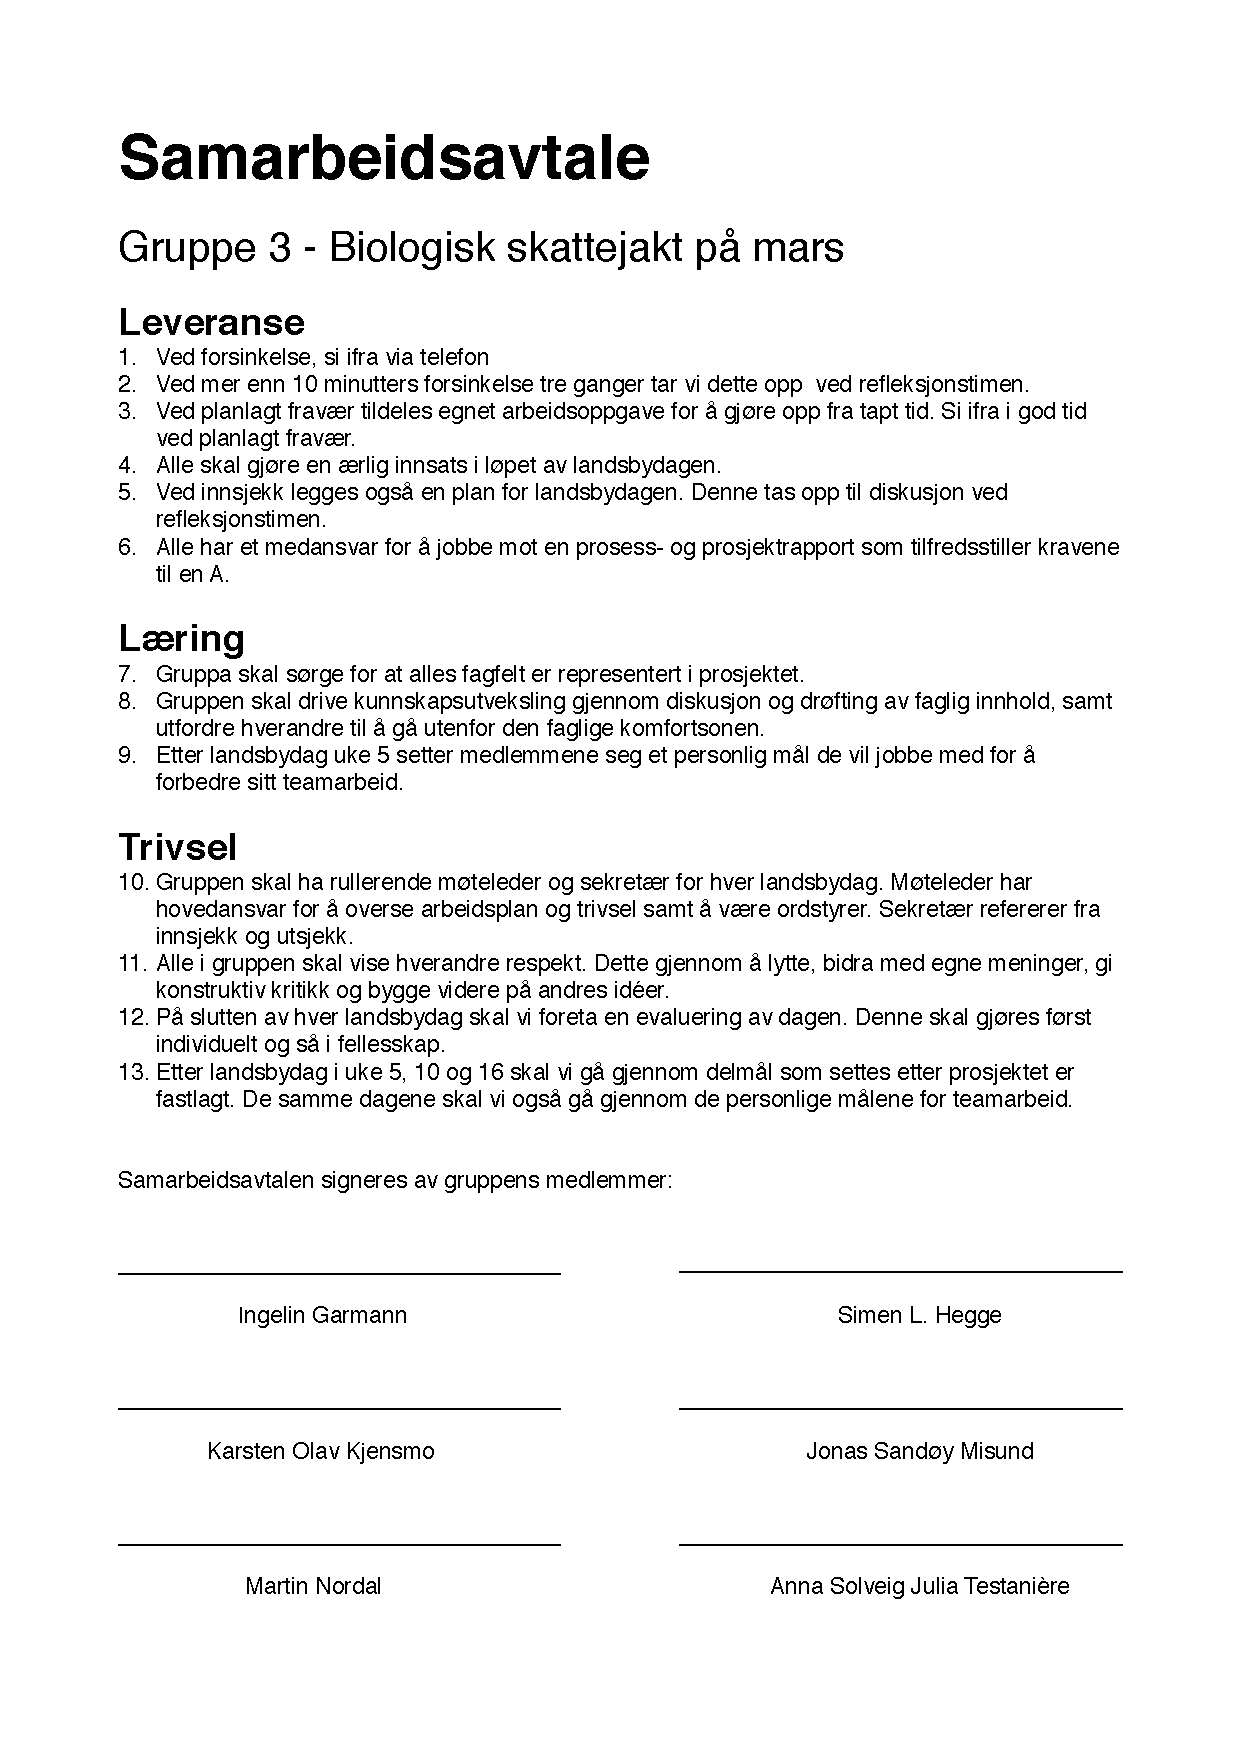
\includegraphics[width=0.9\textwidth]{Samarbeidsavtale.pdf}
\end{center}

\section{Samarbeidsavtale versjon 2}
\label{Ved:samarbeidsavtale_2}
\begin{center}
	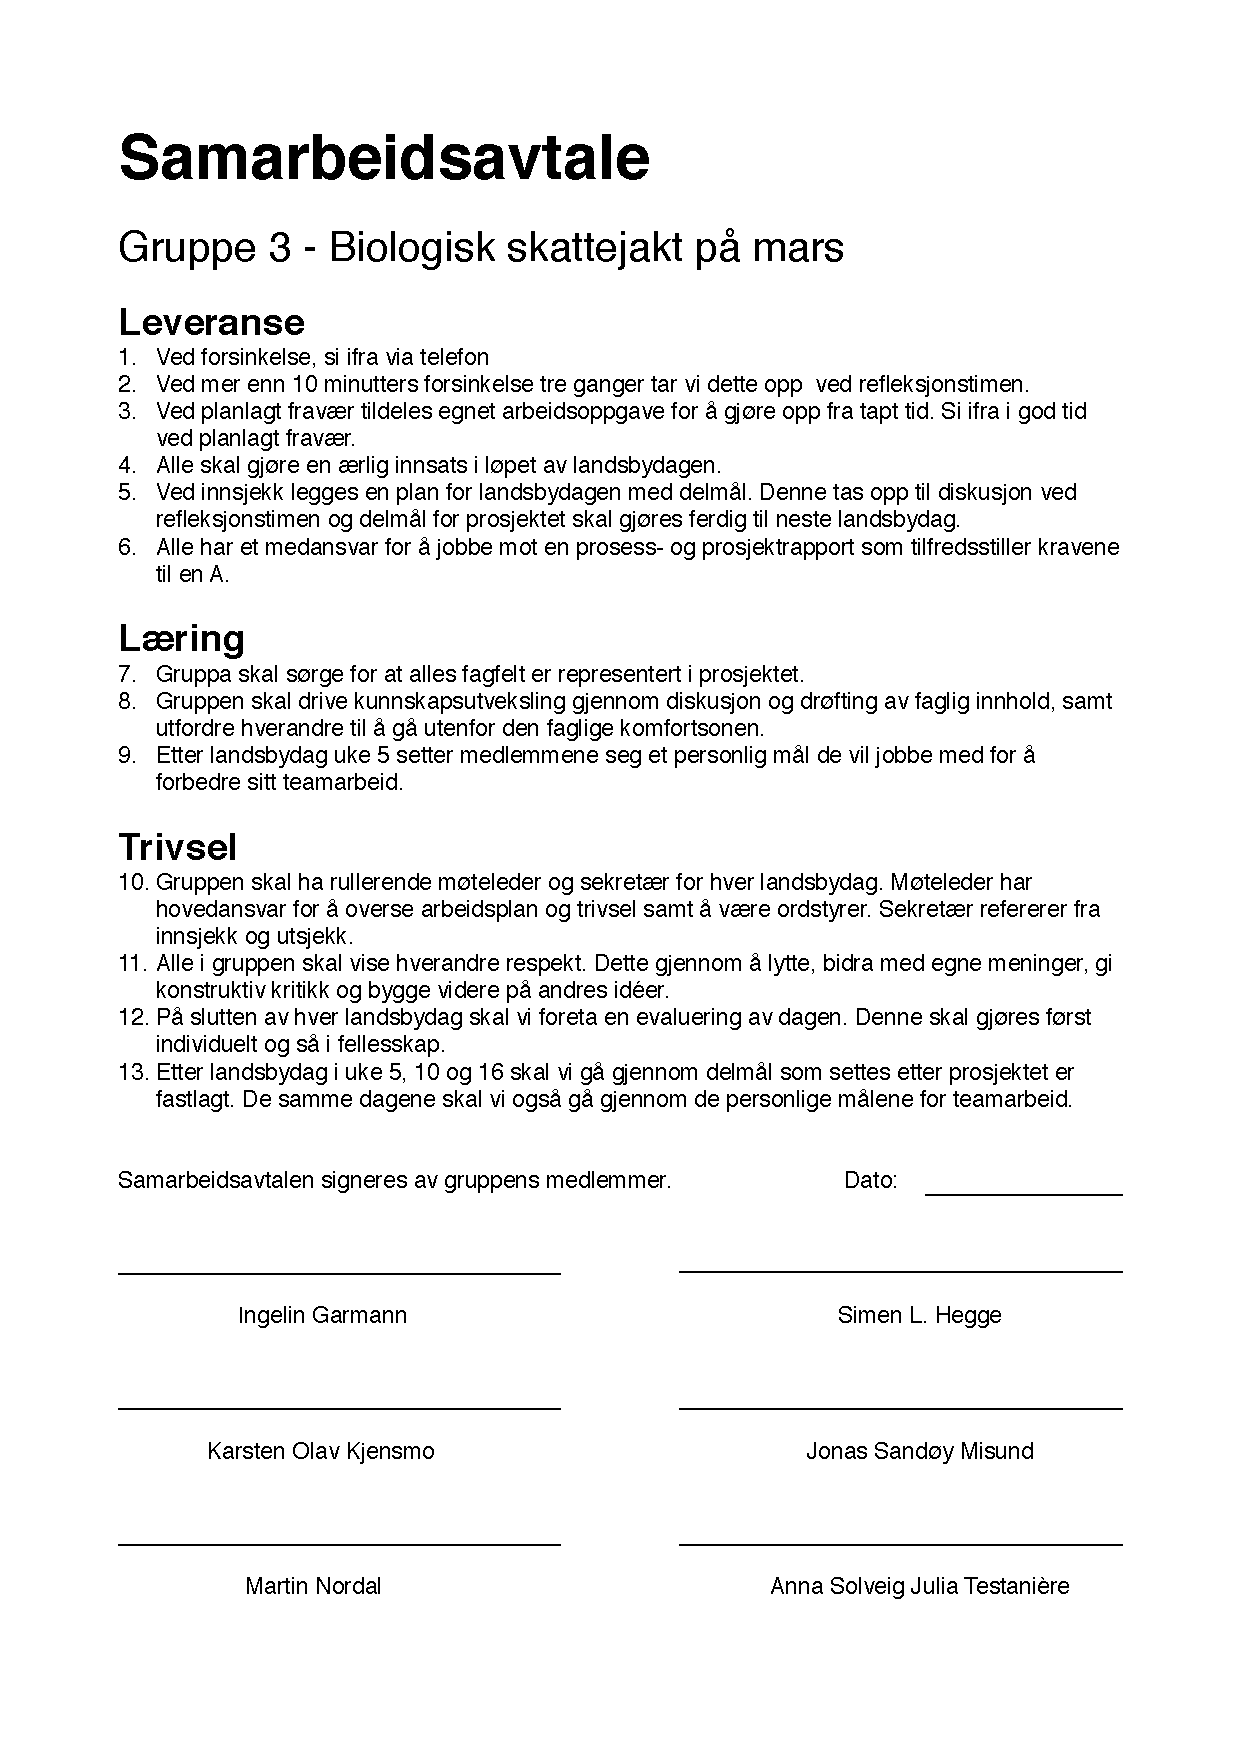
\includegraphics[width=0.9\textwidth]{Samarbeidsavtale_2.pdf}
\end{center}

\end{appendices}

\end{document}